\chapter{Crop development and growth}

\section{Overview of the crop growth model}

The WOFOST model describes phenological development, growth and yield formation of
a crop from emergence till maturity on the basis of crop genetic properties and 
environmental conditions. The model simulates dry matter accumulation of a crop as a function
of irradiation, temperature and crop characteristics in time steps of one day. 
The basis for calculating dry matter production, is the rate of gross CO$_{{\rm 2}}$ assimilation of
the canopy. This rate is dependent on the radiation energy absorbed by the canopy, which
is a function of incoming radiation and of crop leaf area. From the absorbed radiation and
the photosynthetic characteristics of single leaves, the daily rate of CO$_{{\rm 2}}$ assimilation of the
crop is calculated. Part of the carbohydrates produced (CH$_{{\rm 2}}$O) are used to provide energy
for the maintenance of the existing live biomass (maintenance respiration). The remaining
carbohydrates are converted into structural matter. In this conversion, some of the weight
is lost as growth respiration. The growth rate is thus obtained as:

\begin{equation}
% eq 5.1
\Delta W ~=~ C _{e} ~( A ~-~ R _{m} )
\end{equation}

Where:\\[5pt]
\begin{tabularx}{\textwidth}{llXr}
	$\Delta$W &:& Growth rate    &   
	[kg Dry Matter ha$^{{\rm -1}}$ d$^{{\rm -1}}$]\\
	A  &:& Gross assimilation   rate &  
	[kg CH$_{{\rm 2}}$O ha$^{{\rm -1}}$ d$^{{\rm -1}}$]\\
	R$_{{\rm m}}$  &:& Maintenance respiration rate    &  
	[kg CH$_{{\rm 2}}$O ha$^{{\rm -1}}$ d$^{{\rm -1}}$]\\
	C$_{{\rm e}}$ &:& Conversion efficiency off assimilates total crop   &   
	[kg Dry Matter kg$^{{\rm -1}}$ CH$_{{\rm 2}}$O]\\
\end{tabularx}

The dry matter produced is partitioned amongst the various plant organs such as roots,
leaves, stems and storage organs, using partitioning factors that are a function of the
phenological development stage of the crop (Spitters et al., 1989). The fraction partitioned
to the leaves, determines leaf area development and hence the dynamics of light interception. 
The dry weights of the plant organs are obtained by integrating their growth rates
over time (see eq. \ref{eq:euler_integration}).

Leaf mass is subdivided into age classes. During the development of the crop a part of
living biomass dies due to senescence. Some simulated crop growth processes are
influenced by temperature, like for example the maximum rate of photosynthesis and the
maintenance respiration. Other processes like the partitioning of assimilates or decay of
crop tissue are steered by the phenological stage. The phenological development stage is
calculated as a function of ambient temperature and possibly modified by the effect of day
length. An overview of all these processes is depicted in \ref{fig:CropGrowthProc2}.

\begin{figure}[p]
	\centering
	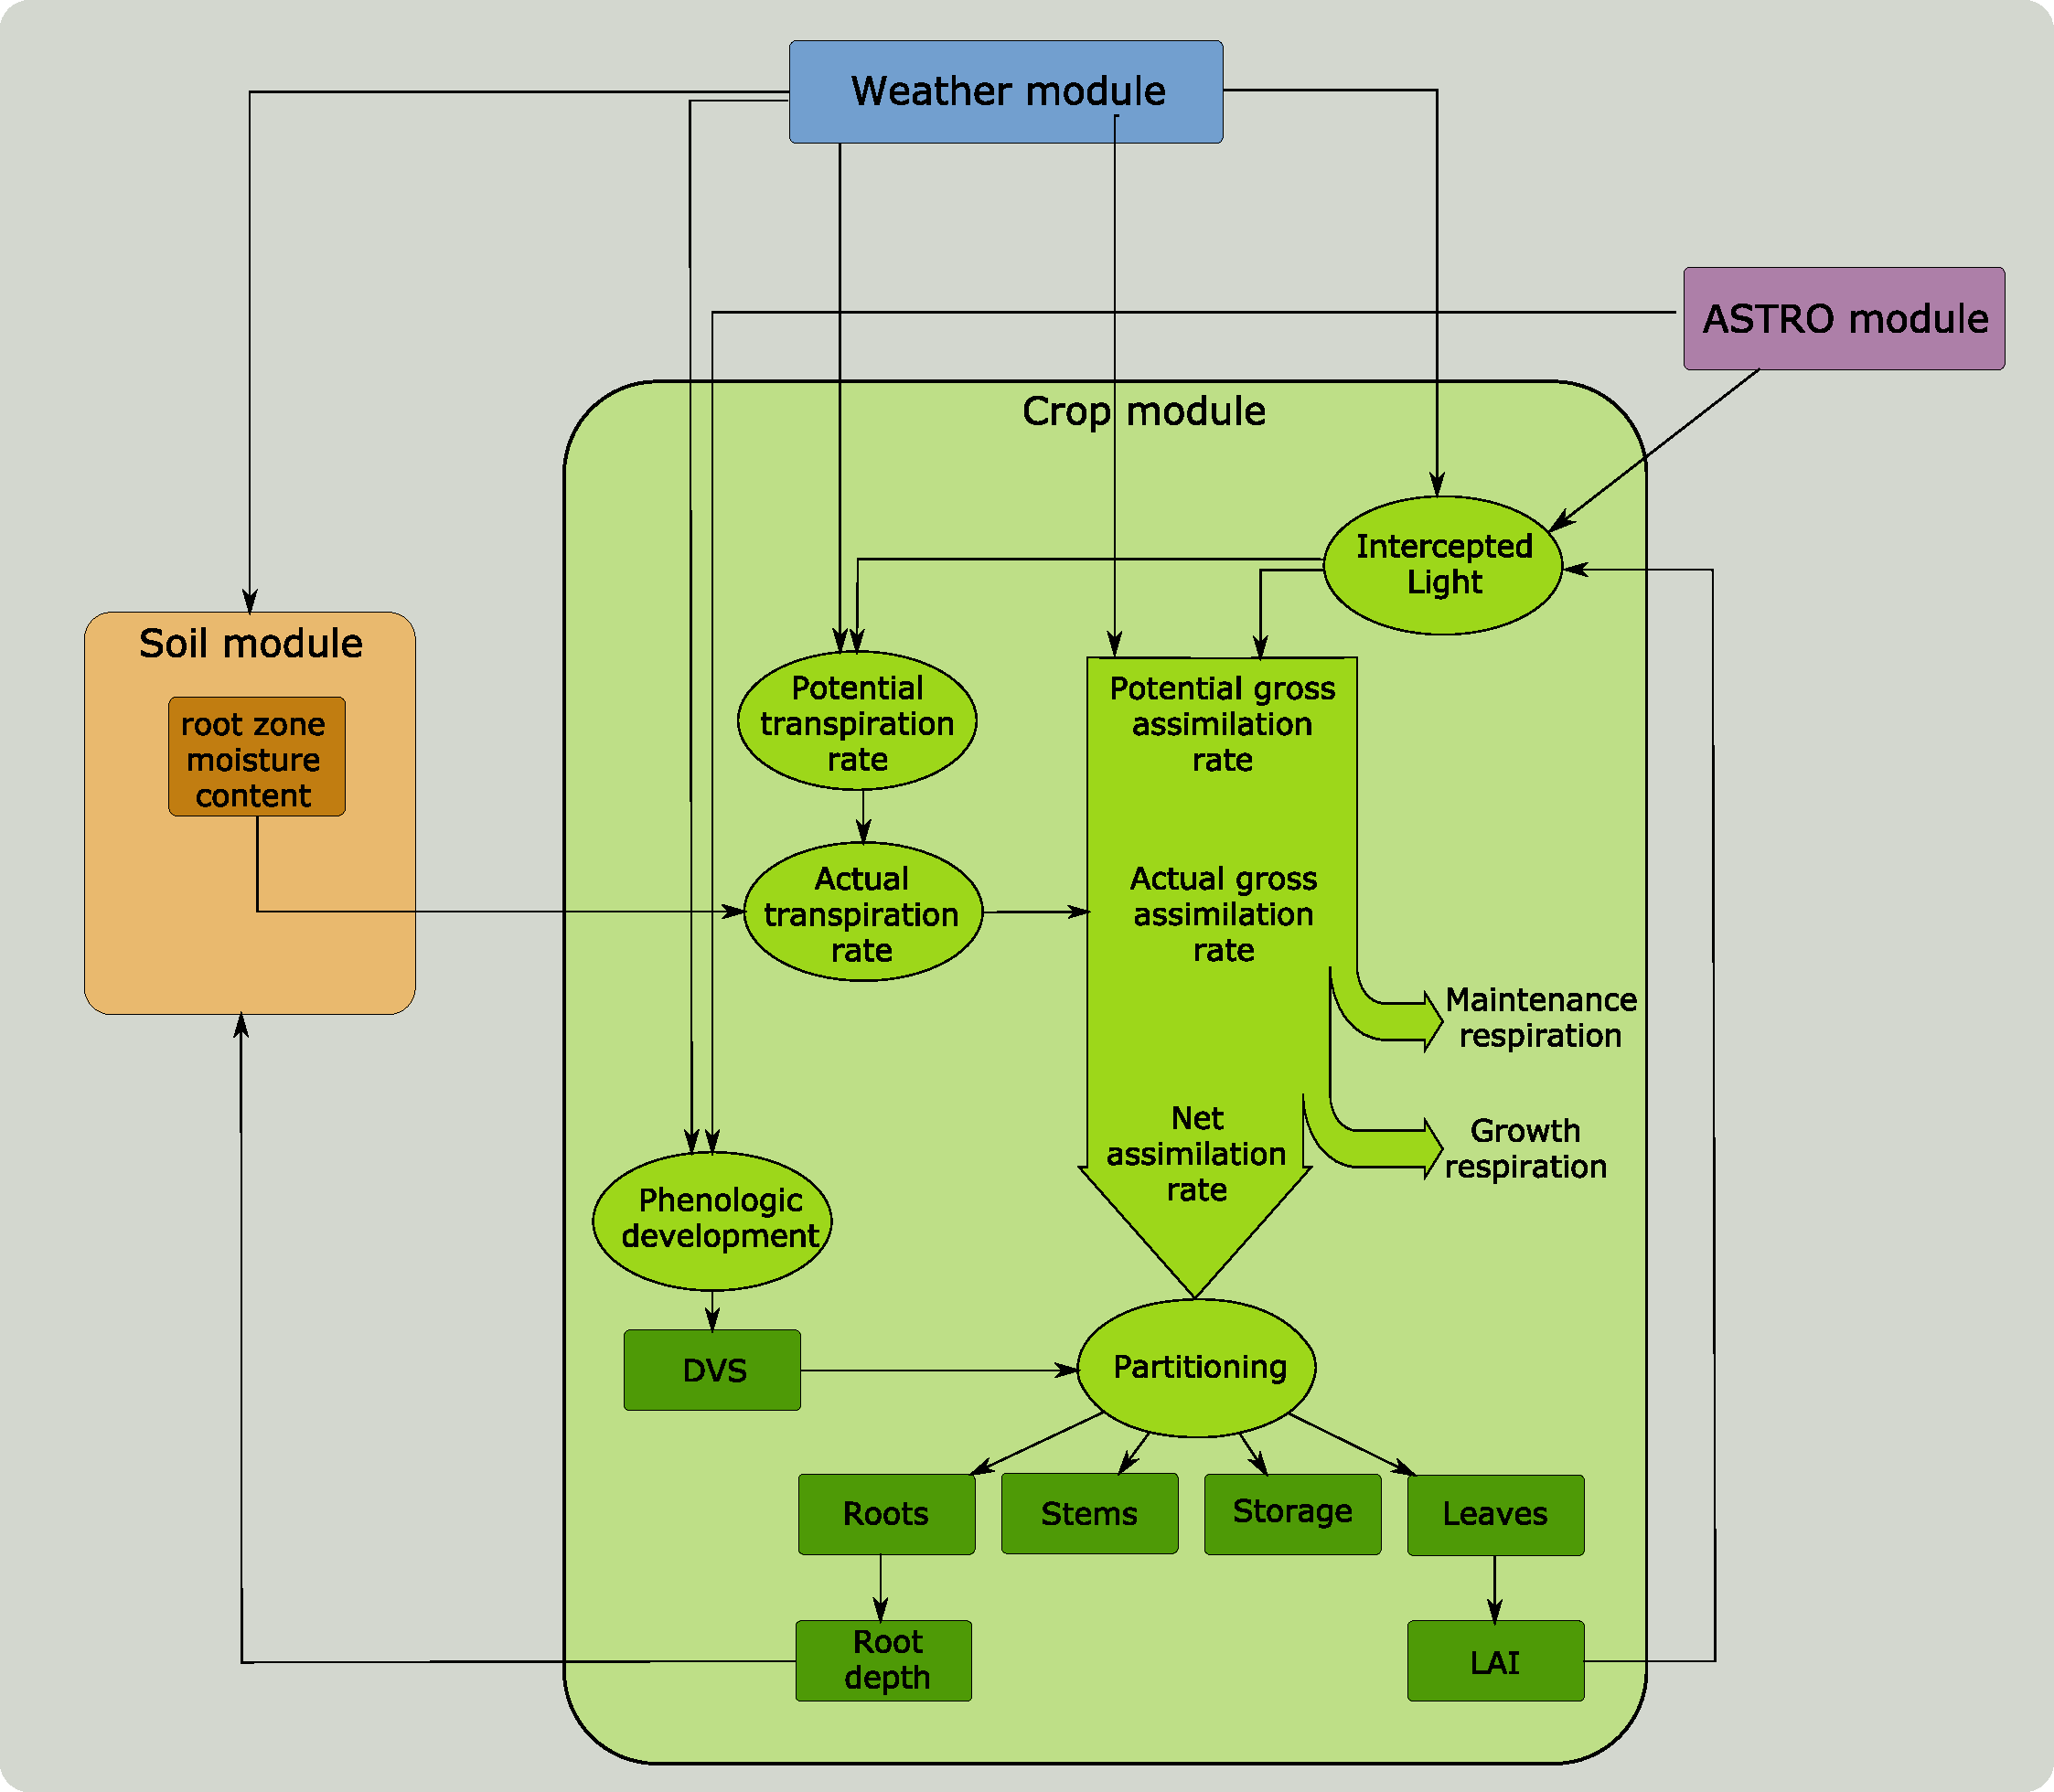
\includegraphics[width=\textwidth ]{\FigDir/wofost_schema_v3.pdf}
	\caption{Schematic overview of the major processes implemented in WOFOST and their linkages.}
	\label{fig:CropGrowthProc2}
\end{figure}

\section{Phenological development of a crop}

The physiological age of a plant is defined by the development stage (DVS), which on its turn is
characterized by the formation of the various organs and their appearance. The most
important phenological change is the one from vegetative to the reproductive stage, which
determines the most important change in the dry matter allocation over organs. As many
physiological and morphological processes change with the phenological stage of the
plant, accurate quantification of phenological development is essential in any simulation
model for crop growth. In WOFOST, the development stage is expressed in a dimensionless variable, 
having the value -0.1 at sowing, 0 at seedling emergence, 1 at flowering and 2 at maturity. 

In recent years the BBCH scale (https://en.wikipedia.org/wiki/BBCH-scale) was developed to provide 
a framework for defining phenological scales for a variety of crops. The phenological stages
used by WOFOST roughly correspond to BBCH scales 0 (sowing), 1 (leaf development), 6 (flowering)
and 9 (senescence). Converting the internal of WOFOST to use the BBCH scale for phenology is 
not trivial because many WOFOST parameters are defined as a function of DVS. Nevertheless,
in calibration studies it was demonstrated that specific DVS values can be linked consistently
to specific BBCH stages. Although the exact DVS values for a crop to reach a specific BBCH
stages can be variety specific.


\subsection{Crop emergence}

As start of the growing season the date of sowing or of emergence can be chosen. For a
photosynthesis-driven model like WOFOST, the simulation of crop growth starts at
emergence. If the sowing date is chosen by the model user, the day of emergence is
determined by the model. The crop emergence can be
defined as a function of the effective daily temperature sum since sowing date. Emergence
takes place when the effective daily temperature sum reaches the threshold temperature
for emergence (acronym: {\bf TSUMEM}). This threshold temperature is crop specific and
should be given by the user. The daily effective temperature depends on the base
temperature {\bf TBASEM}, below which no germination processes take place, and the maximum daily
temperature, beyond which the germination activity does not increase anymore {\bf TEFFMX}.
Both are crop specific. An example of this effective daily temperature as a function of daily
average temperature is depicted in figure \ref{fig:TEFFMAX}.

\begin{figure}[p]
	% fig 5.2
	\centering
	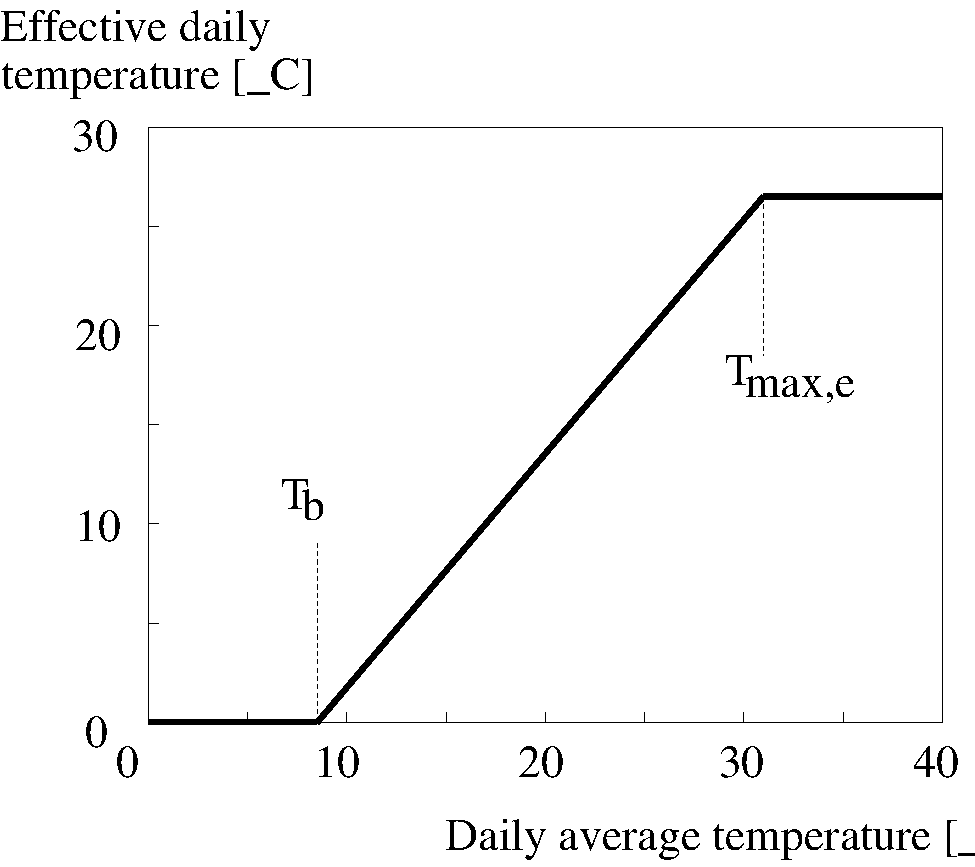
\includegraphics[width=120mm]{\FigDir/TEFFMAX.pdf}
	\caption{Effective temperature from sowing to emergence} 
	\label{fig:TEFFMAX}
\end{figure}

The following relationship can be defined for the effective temperature sum:

\begin{align}
T_{e} &= 0            & T \le T _{b} \nonumber  \\
T_{e} &= T~-~ T _{b}  & T _{b} ~<~T ~ < ~T _{\max ,e} \nonumber  \\
T_{e} &= T _{\max ,e} & T _{b} T \ge  T _{\max \, ,\, e}
\end{align}

Where:\\[5pt]
\begin{tabularx}{\textwidth}{llXr}
	T$_{{\rm e}}$ &:& Effective daily temperature & 
	[\degrees C]\\
	T$_{{\rm max,e}}$ &:& Maximum temperature beyond which phenological 
	activity does not increase    &    [\degrees C]\\
	T$_{{\rm b}}$ &:& Base temperature below which phenological development stops & 
	[\degrees C]\\
	T  &:& (Average) daily temperature & [\degrees C]
\end{tabularx}

Species originating from temperate regions show a base temperature of
0$-$3\degrees C, while species of subtropical and tropical origins have a base temperature of
9$-$14\degrees C (Angus {\it et al.}, 1981). Within a species, cultivars may vary substantially 
in their temperature requirements. The temperature sum, therefore, must be characterized for
each cultivar or group of cultivars (maturity classes).   

\subsection{Phenological development stage}
\label{sec:DVS}

A crop passes through successive phenological development stages. In WOFOST these stages 
are expressed in degree-days and defined by two parameters. The TSUM1 parameter defines
the number of degree-days for the emergence-anthesis period, while the TSUM2 parameter
defines the number of degree-days for the anthesis-maturity period. 
The length of these in days stages depends on the development rate. Development rates are 
controlled by vernalization requirements, day length and/or temperature. In the model before
anthesis, all factors can be active. After anthesis only temperature influence is possible.

Temperature is the main environmental factor affecting the development rate. Higher
temperatures increase the development rate leading to shorter growing periods. This rate
responds to temperature according to a curvilinear relationship. However, it has often
been demonstrated, that over a wide range of temperatures, the development rate
increases more or less linearly with temperature (van Dobben, 1962; van Keulen \&
Seligman, 1987).

In the model a flexible relation is used where the effective increase in temperature
sum, used for the calculation of the development rate, is dependent on the daily temperature 
(Summerfield \& Roberts, 1987). This relation is specified in an AFGEN table, 
allowing to account for non-linearity (lower and upper threshold values and optimum
ranges). The average temperature is the independent variable in the AFGEN table (see
Appendix 2). 

The development rate based on temperature can be reduced by the effect of vernalization and 
day length and can thus be obtained by:

\begin{equation}
% eq 5.3
\label{eq:5.3}
D_{r,t} = {f_{vern}}{f_{dayl}}{\frac{DT_{s}}{\sum T_{i}}}
\end{equation}

Where:\\[5pt]
\begin{tabularx}{\textwidth}{llXr}
	$f_{{\rm vern,t}}$ &:& Reduction factor for vernalization at time step t  & [-]\\
	$f_{{\rm dayl,t}}$ &:& Reduction factor for day length at time step t  & [-]\\
	D$_{{\rm r,t}}$ &:& Development rate at time step t  & [d$^{{\rm -1}}$]\\
	DT$_{{\rm s}}$ &:& Daily effective temperature & [\degrees C]\\
	$\sum$T$_{{\rm i}}$ &:& Temperature sum required to complete stage i & [\degrees C d]\\
\end{tabularx}

The temperature dependent correction factor, {\bf DT$_{{\rm s}}$} (acronym: {\bf DTSMTB}) and 
the temperature sum required to complete stage i, {\bf $\sum$T$_{{\rm i}}$} (acronym: 
{\bf TSUM1} or {\bf TSUM2}) are crop dependent and should be provided by the user.

The development stage at time step t is the integral of the development rate over the time
(i.e. time span from emergence to current time step) and can be calculated according to:

\begin{equation}
\label{eq:5.4}
D_{s,t} ~=~ D_{s,t-1} + D_{r,t} \Delta t
\end{equation}

Where:\\[5pt]
\begin{tabularx}{\textwidth}{llXr}
	D$_{{\rm s,t}}$ &:& Development stage at time step t    &    [-]\\
	D$_{{\rm r,t}}$ &:& Development rate at time step t     &   [d$^{{\rm -1}}$]\\
	$\Delta$t &:& Time step   &     [d]\\
\end{tabularx}

\subsection{Day length}

For certain crops or cultivars, during the vegetative stage (i.e. D$_{{\rm s}}$ $<$ 1), the 
effect of day length should be taken into account (e.g. "photosensitivity"). Moreover, crops 
that are sown in autumn
in temperate climate often require exposure to the prolonged cold of winter in order to be
able to flower. This effect is called the "vernalization requirement" of the crop.

Approaches that describe the effect of day length 
quantitatively are given amongst others by  Weir {\it et al.} (1984), Hadley {\it et al}. (1984) 
and Reinink {\it et al.} (1986). In WOFOST, a reduction factor for the development rate as a 
function of the day length is introduced. In case of photosensitivity can be calculated as:

\begin{equation}
\label{eq:5.5}
f_{red} ~=~{\frac{D ~-~D _{c} }{D _{o} ~-~ D _{c} }} ~~~~~~~~~0~\le ~f _{red} ~\le ~1
\end{equation}

Where:\\[5pt]
\begin{tabularx}{\textwidth}{llXr}
	$f_{{\rm dayl}}$ &:& Development rate reduction factor as function of day length   &     [-]\\
	D &:& Present day length (see eq. \ref{eq:AstroDaylength})   &     [h]\\
	D$_{{\rm c}}$ &:& Critical day length for development (lower threshold)    &    [h]\\
	D$_{{\rm o}}$ &:& Optimum day length for development (upper threshold)    &    [h]\\
\end{tabularx}

The user should provide information whether the development rate depends on temperature, 
on day length or on temperature and day length (acronym: {\bf IDSL}). The critical
daylength, {\bf D$_{{\rm c}}$} (acronym: {\bf DLC}) and the optimum daylength, 
{\bf D$_{{\rm o}}$} (acronym: {\bf DLO}) are crop dependent and should also be provided by 
the user. 

Note that in modern cultivars, photosensitivity is much less pronounced than in traditional
cultivars, and that for the purpose of modelling the day length influence can often be ignored.
However, for winter crops influence of day length and vernalization must be taken into
account in order to avoid that the choice of the sowing date in autumn has a large impact on 
the flowering and maturity date of the crop.


\subsection{Vernalization}

Vernalization is the induction of a plant's flowering process by exposure to the prolonged cold of winter, or by an artificial equivalent. After vernalization, plants have acquired the ability to flower, but they may require additional seasonal cues or weeks of growth before they will actually flower (source: Wikipedia). 

In WOFOST vernalization is simulated by assuming that a crop requires a number of (cultivar-specific)
cold days in order to reach its vernalization requirement. One cold day is added to the vernalization state 
when the daily average temperature is within the optimal temperature range for vernalization. A fractional
day or zero  is added when the temperature is outside of this range. This is rate of vernalization
(acronym: {\bf VERNR}) is decribed using an AFGEN table (acronym:  {\bf VERNRTB}) which describes the
temperature response curve for vernalization (figure ???).

The reduction factor on development rate is than derive by linearly scaling the current vernalization state 
((acronym:  {\bf VERN}))  between a base vernalization ((acronym:  {\bf VERNBASE})) and the number of 
days required to saturate the vernalization requirement (acronym:  {\bf VERNSAT}). The reduction 
factor can thus be expressed as: 

\begin{equation}
\label{eq:vern_factor}
f_{vern} ~=~{\frac{V ~-~V_{base} }{V _{sat} ~-~ V_{base} }} ~~~~~~~~~0~\le ~f _{vern} ~\le ~1
\end{equation}



Note that it is possible for crops under certain conditions to de-vernalize, but this effect is not taken
into account in WOFOST.

\subsection{End of the crop cycle}

The simulation of crop growth stops when the development stage reaches the stage at
which the crop will be harvested (acronym: {\bf DVSEND}). For crops that are harvested
at maturity {\bf DVSEND}) will be equal to 2.0. However, for crops that are deliberately
harvested earlier (e.g. silage maize) the value can be lower. For crops that are harvested
at a defined date, the value for {\bf DVSEND}) will be ignored.
